\documentclass{jsarticle}
\usepackage[dvipdfmx]{graphicx}
\usepackage{subcaption}
\captionsetup[figure]{justification=centering}
\captionsetup[table]{justification=centering}
\usepackage[ipa]{pxchfon}
\usepackage{float}
\usepackage[margin=20truemm]{geometry}


\begin{document}
\title{{\vspace*{-10mm}}{\LARGE 0622課題(EKFの実習)}}
\author{\large 千葉工業大学 先進工学部 未来ロボティクス学科 \vspace*{4mm}\\20C1015 今井悠月}
\date{}
\maketitle\vspace*{10mm}
\vspace*{-10mm}

\section*{問}
時間に対する『位置』と EKF で求めた『位置の平均』『分散』を折れ線グラフ(散布図)で表し, Rt, Qtを
変更\hspace*{1zw}してどのように推定値が変化するかを確認せよ.

\section*{解答}

\begin{figure}[H]
  \centering
   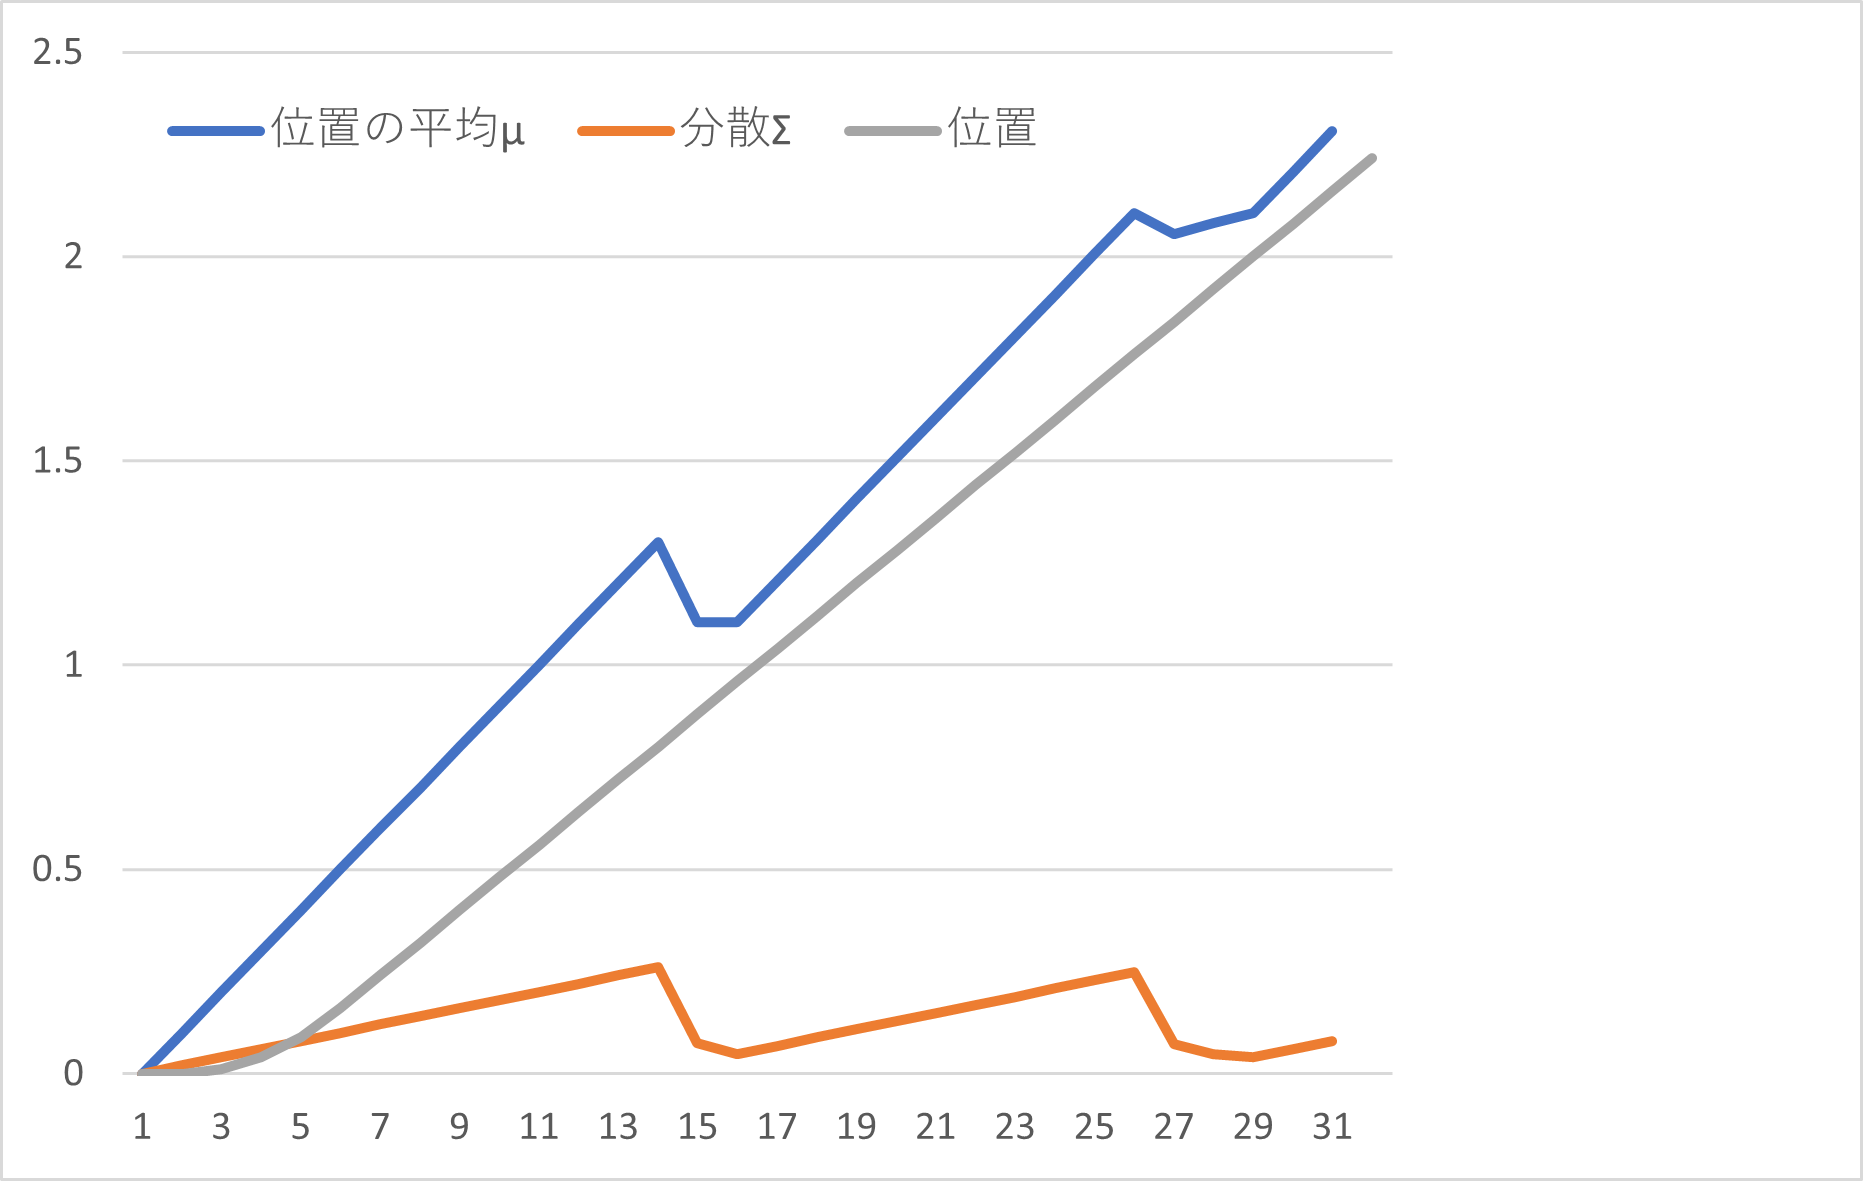
\includegraphics[scale=0.15]{./fig/def.png}
   \caption{デフォルト値(Rt = 0.02, Qt = 0.1)の時のグラフ}
\end{figure}

\begin{figure}[H]
  \centering
   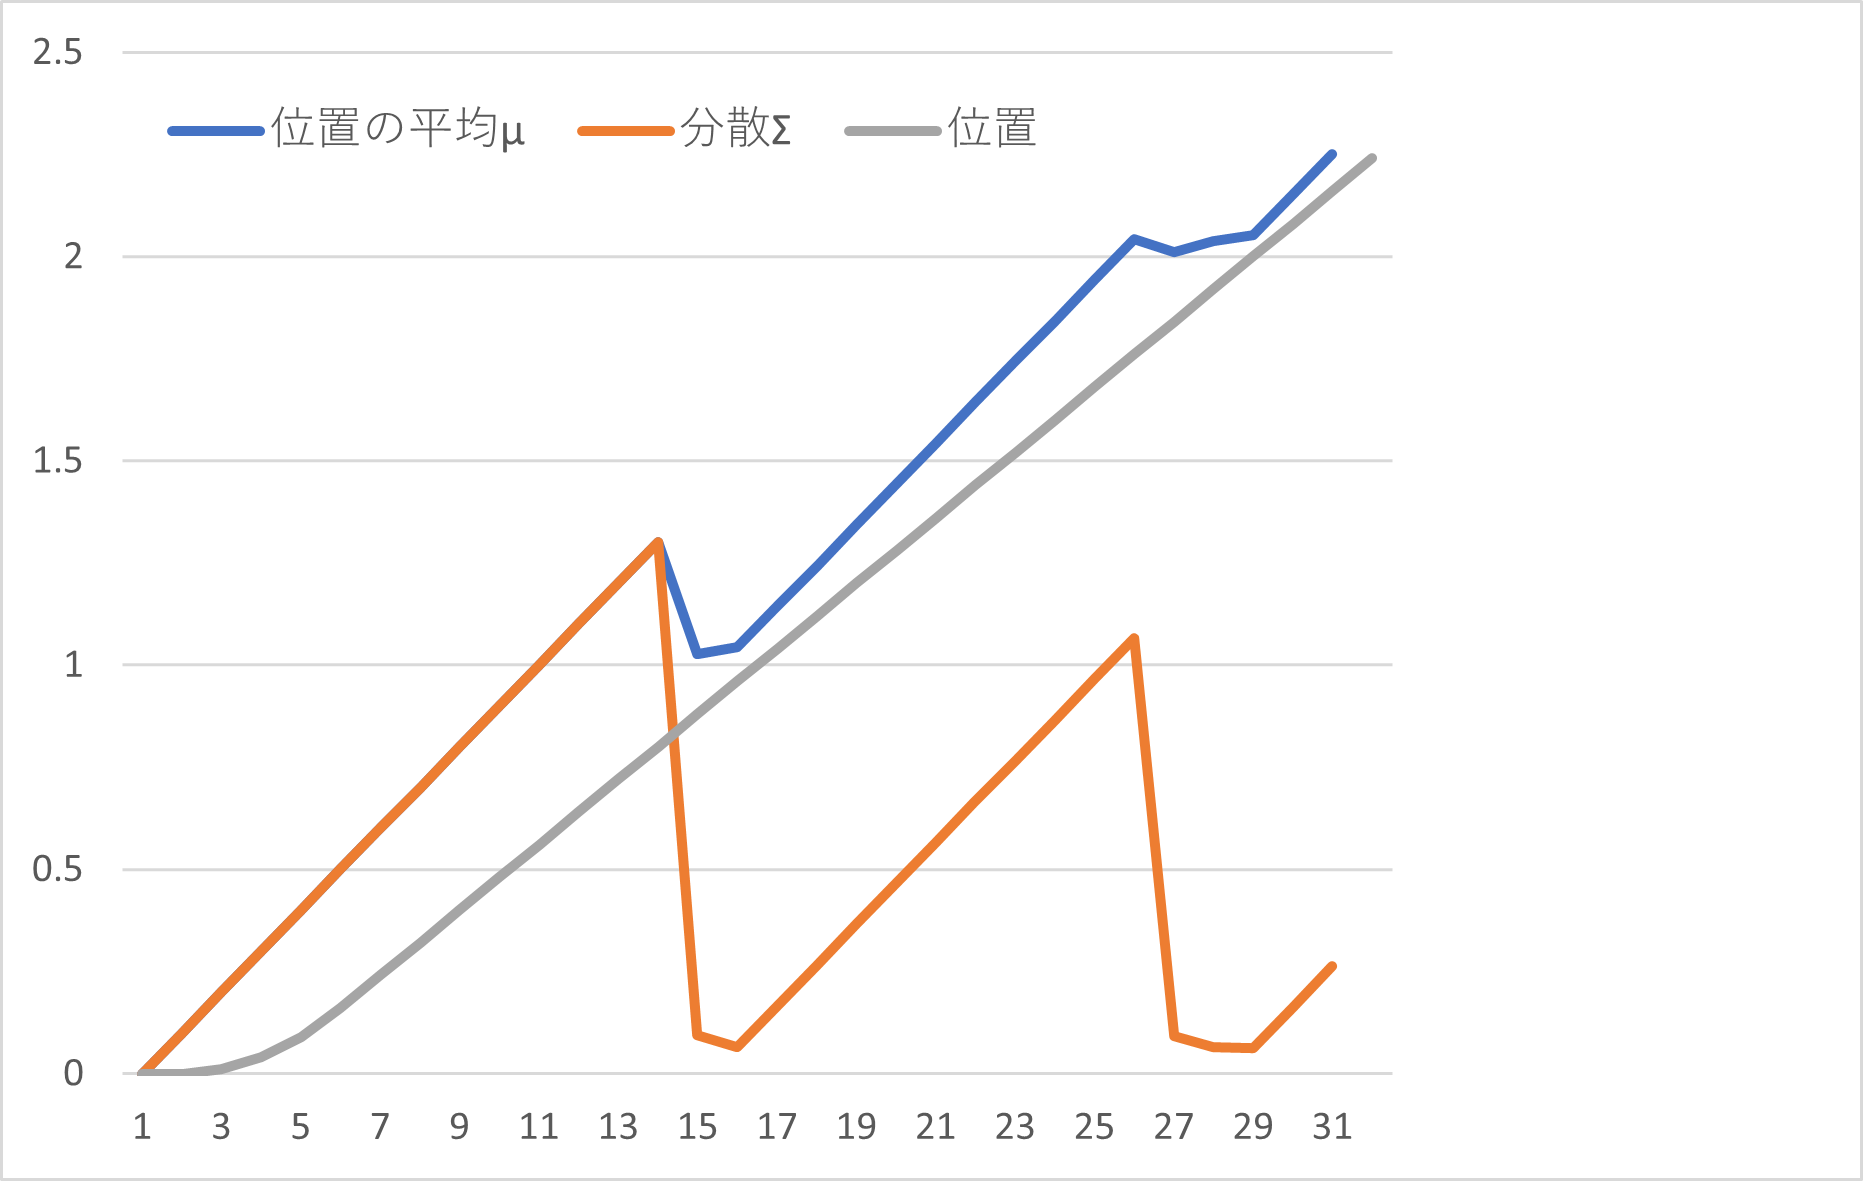
\includegraphics[scale=0.15]{./fig/R=0.1.png}
   \caption{Rt = 0.1, Qt = 0.1の時のグラフ}
\end{figure}

\begin{figure}[H]
  \centering
   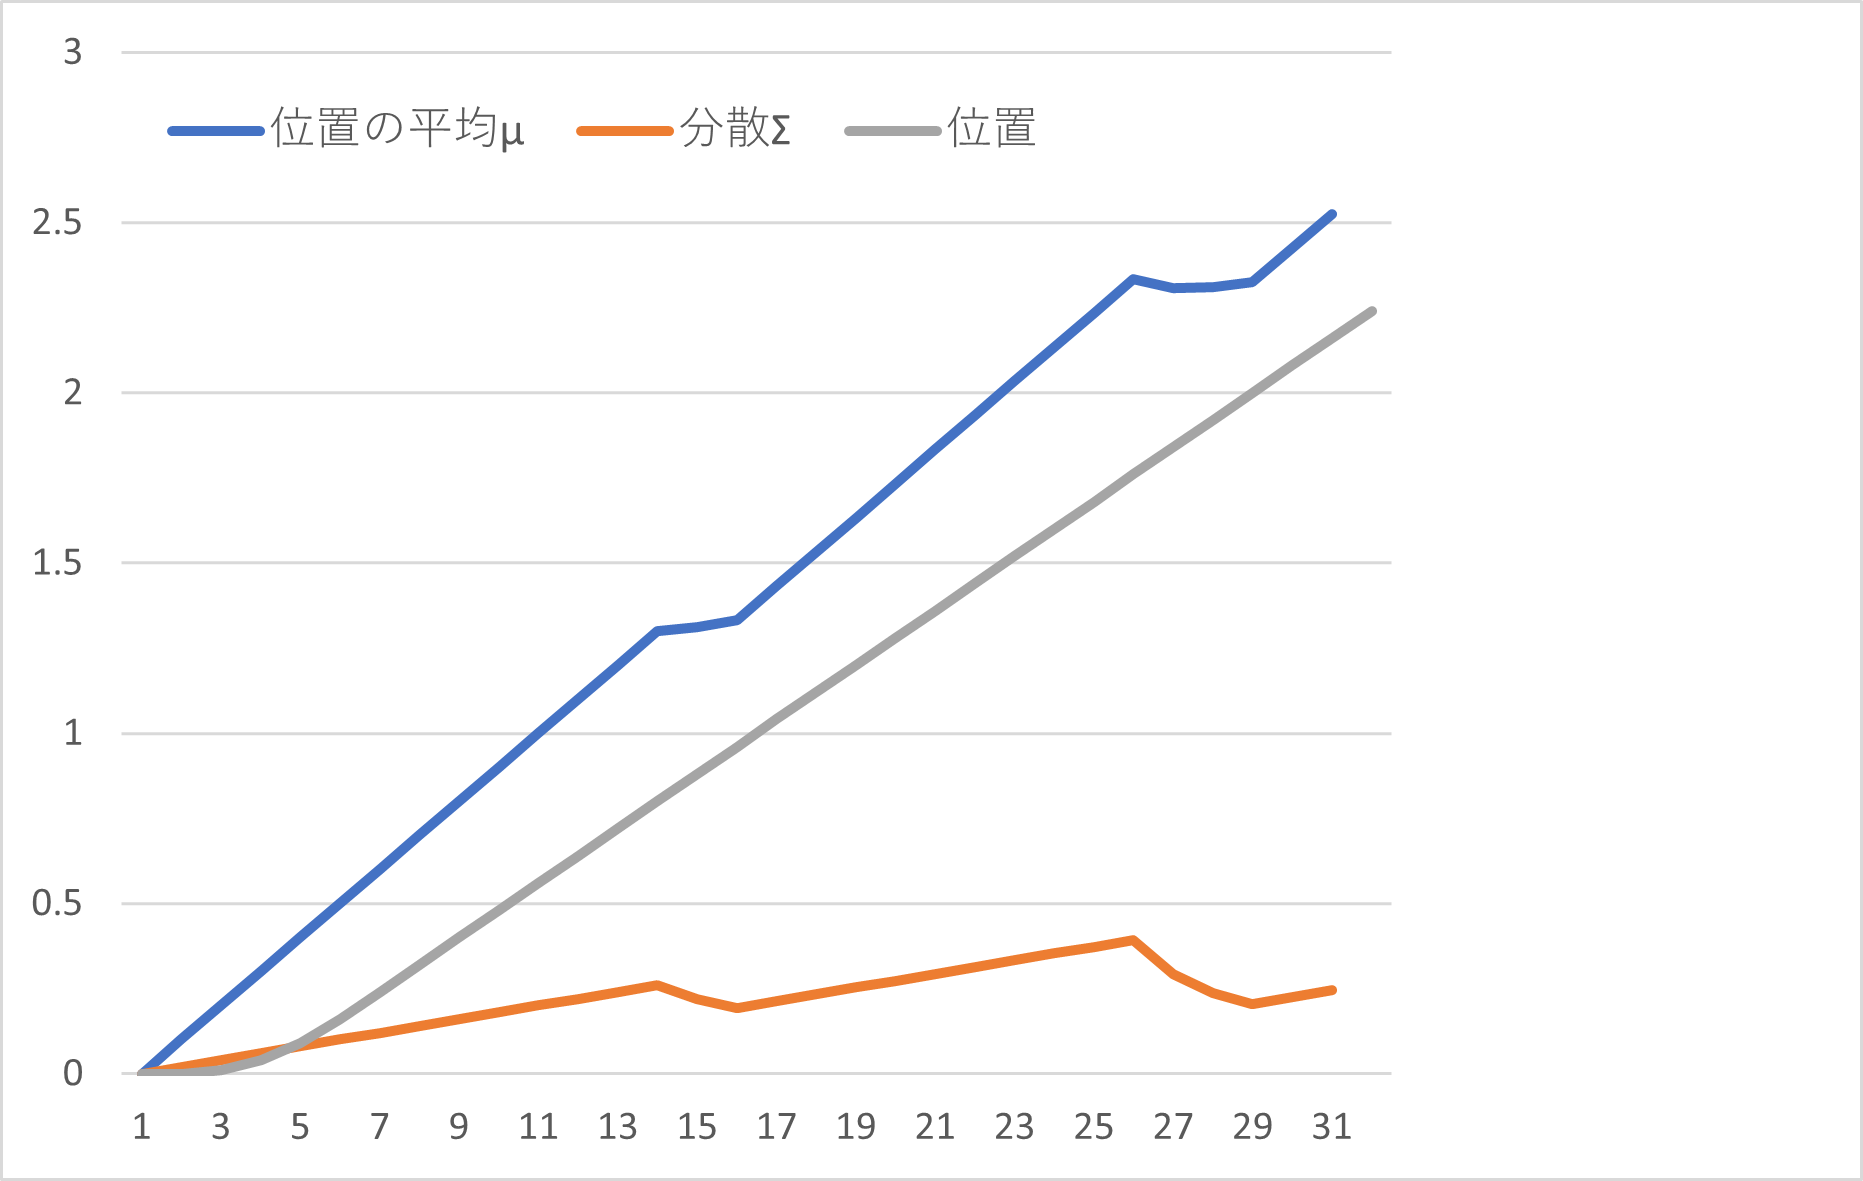
\includegraphics[scale=0.15]{./fig/Q=1.png}
   \caption{Rt = 0.02, Qt = 1の時のグラフ}
\end{figure}

\begin{figure}[H]
  \centering
   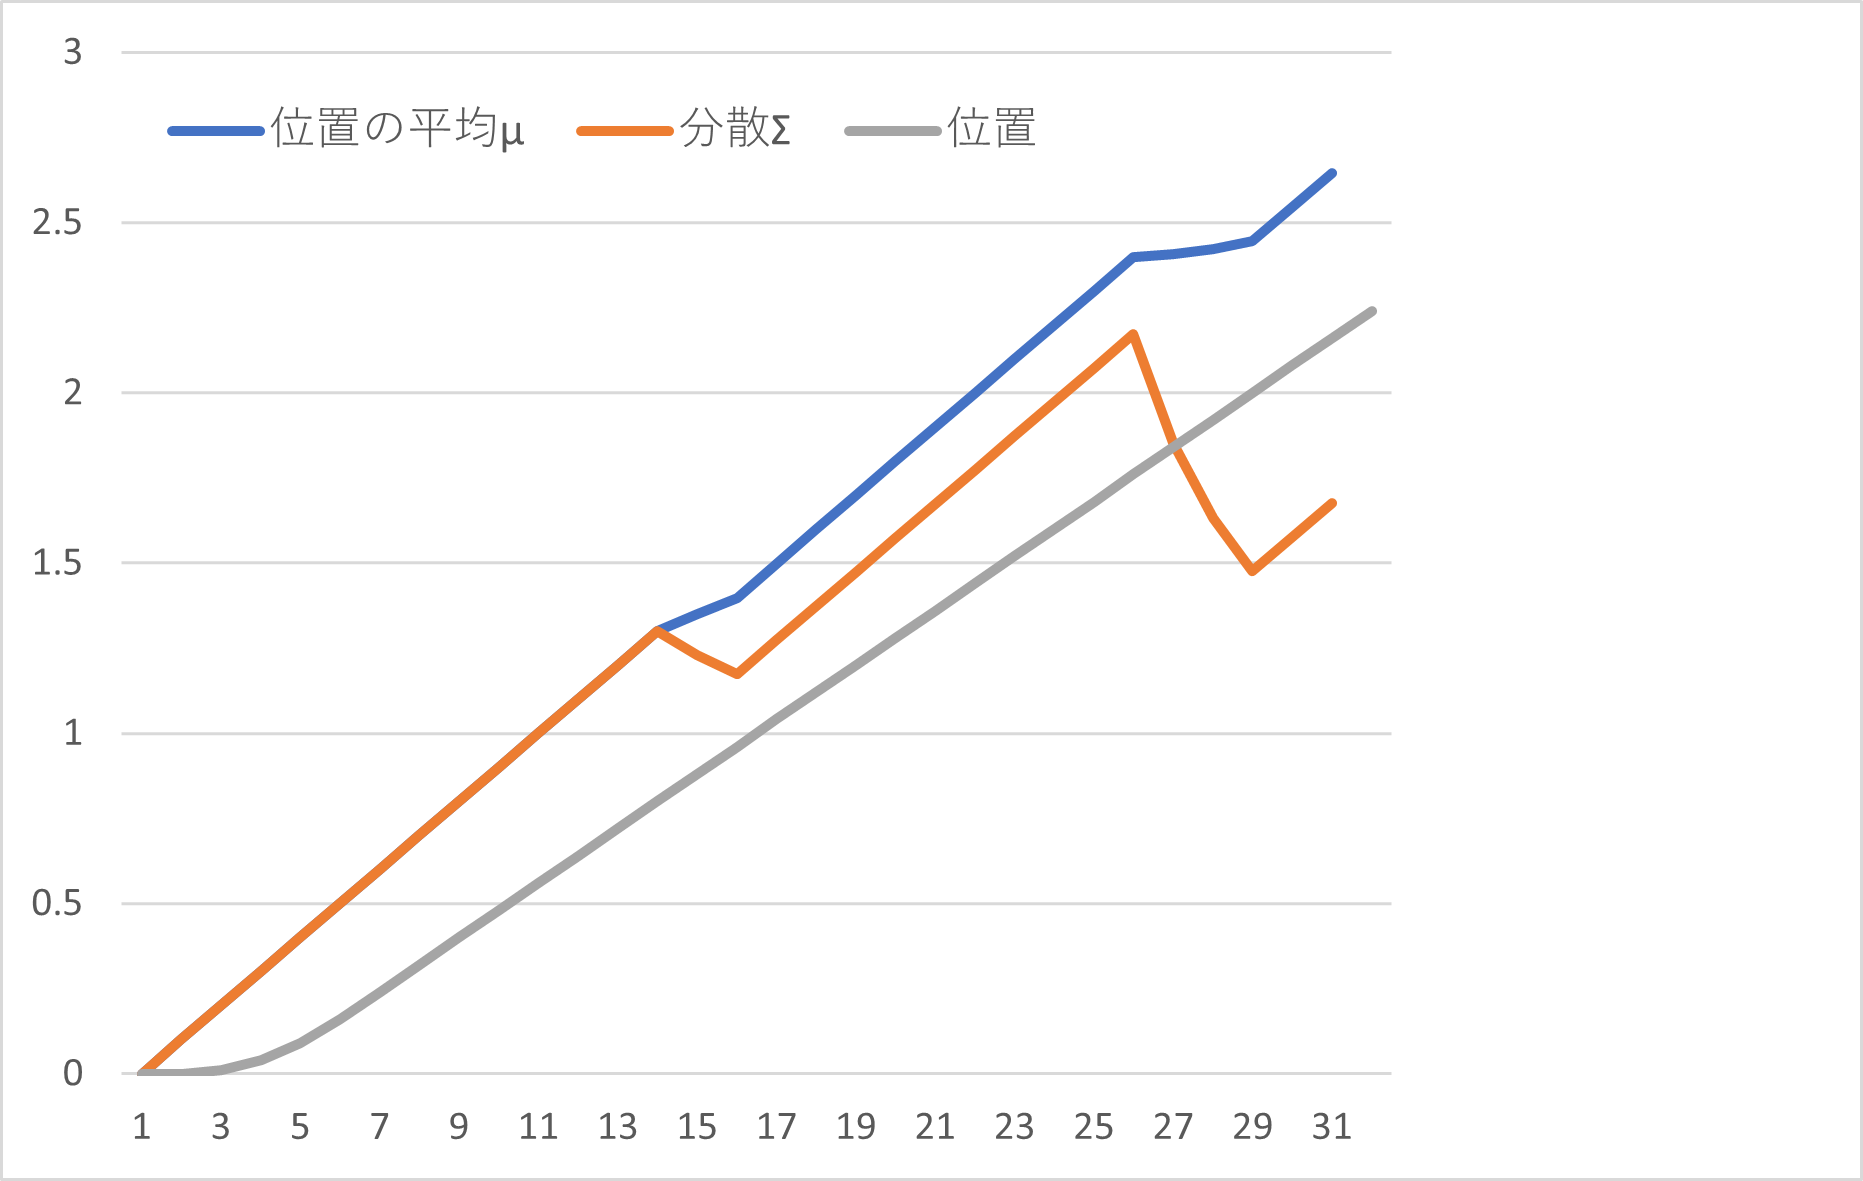
\includegraphics[scale=0.15]{./fig/R=0.1_Q=10.png}
   \caption{Rt = 0.1, Qt = 10の時のグラフ}
\end{figure}

\subsection*{コメント}
図1と図2を比較すると, 図2のグラフは共分散が大きくなっていることがひと目でわかる.
つまり, 図2の場合, 推定値の不確かさが高まっている. よって, 推定値の信頼度は低い.
図3を見ると, それなりに共分散は小さいものの, デフォルト値である図1の方が全体的に小さくなっている.
図4は全体的に共分散が大きくなっているため, 信頼度は低い. これらの結果から, デフォルト値のグラフの概形が良く, 
Rt, Qtは小さな値のほうが良いのではないかと考えられる.
\end{document}